% !TEX TS-program = xelatex
% !TEX encoding = UTF-8 Unicode
% !Mode:: "TeX:UTF-8"

%\documentclass[bachelor]{dutthesis} % 本科
%\documentclass[master]{dutthesis} % 硕士
\documentclass[doctor]{dutthesis} % 博士
\usepackage{amsmath}
\usepackage{amsfonts} 
\usepackage{bm} 
\usepackage{algorithm}
\usepackage{algorithmicx}
\usepackage{algpseudocode}
\usepackage{subfigure}
\usepackage{tabularx}
\usepackage{arydshln}
\usepackage{array}
\usepackage{physics}
\usepackage{enumerate,paralist} %产生列表,有序,缩进等功能
\usepackage{layouts} %用于绘制页面布局
\usepackage{layout} %用于绘制页面布局
\usepackage{listings} %插入代码用,不用可以取消
\lstset{frame=tlrb,fontadjust=true,basicstyle=\fontsize{10}{9}\ttfamily,
emphstyle=\color{red!80},
emph={root,base},emphstyle={\color{blue}},
tab=\rightarrowfill,keywordstyle={[1]\color{blue!80}},
keywordstyle={[2]\color{red!50}},
stringstyle=\color{magenta},
breaklines=true,
columns=fixed,
commentstyle=\color{black!50}}
 

%%%%%%%%%%%%%%%%%%%%%%%%%
%  使得layout使用mm做单位,不重要  %
%%%%%%%%%%%%%%%%%%%%%%%%%
\makeatletter
\renewcommand*{\lay@value}[2]{%
  \strip@pt\dimexpr0.351459\dimexpr\csname#2\endcsname\relax\relax mm%
}
\makeatother

\floatname{algorithm}{算法}
\renewcommand{\algorithmicrequire}{\textbf{输入:}}
\renewcommand{\algorithmicensure}{\textbf{输出:}}
 % 这里是导言区
\begin{document}
\categorynumber{000} % 分类采用《中国图书资料分类法》
\UDC{000}            %《国际十进分类法UDC》的类号
\secretlevel{公开}    %学位论文密级分为"公开"、"内部"、"秘密"和"机密"四种
\studentid{11402004}   %学号要完整,前面的零不能省略。

\title{大连理工大学毕业论文模板-- \TeX}{}{The Format Criterion of Dissertation of 
DUT}{subtitle}
%%%%%%%%%%%%%%%%%%%%%%%%%%%%%%%%%%%%%%%%%%%%%%%%%%%%%%%%%%%%%%
%  title包含四个定义,分别是中文题目,中文副标题,
%英文标题,以及英文副标题,没有副标题可以空{}不能不写
%
%%%%%%%%%%%%%%%%%%%%%%%%%%%%%%%%%%%%%%%%%%%%%%%%%%%%%%%%%%%

\author{三分道人}{Mou Xun}
\advisor{菩提}{祖师}{Puti}{Master}
%		\coadvisor{副导师}{副教授}{Co-advisor's Name}{Associate Prof.} % 没有

\degree{物理博士} % 详细学位名称
\major[12em]{理论物理}
\defenddate{答辩日期}
\authorizedate{学位授予日期}
\department{物理学院}{school of physics}
\duration{2010年9月—201年6月}
\address{物理系}
\maketitle

\begin{abstract}{写作规范;排版格式;博士学位论文 }
大连理工大学博士研究生撰写学位论文应当符合写作规范和排版格式的要求,以下格式为研究生院依据国家标准和行业规范所编制的博士学位论文模板,供博士研究生参照使用。 

摘要部分说明:
“摘要”是摘要部分的标题,不可省略。

标题“摘要”选用模板中的样式所定义的“摘要”;或者手动设置成字体:黑体,居中;字号:小三;1.5倍行距,段前为0行,段后1行。

论文摘要是学位论文的缩影,文字要简练、明确。内容要包括目的、方法、结果和结论。单位制一律换算成国际标准计量单位制,除特殊情况外,数字一律用阿拉伯数码。文中不允许出现插图,重要的表格可以写入。

摘要正文选用模板中的样式所定义的“正文”,每段落首行缩进2个汉字;或者手动设置成每段落首行缩进2个汉字,字体:宋体,字号:小四,行距:多倍行距 1.25,间距:前段、后段均为0行,取消网格对齐选项。

摘要的主要内容为,简述全文的目的和意义、采用方法、主要研究内容和结论。

篇幅以一页为限,摘要正文后列出3-5个关键词,关键词与摘要之间空一行。

“关键词:”是关键词部分的引导,不可省略,黑体,小四。

关键词请尽量用《汉语主题词表》等词表提供的规范词。关键词之间用分号间隔,末尾不加标点。

\end{abstract}

\begin{englishabstract}{Greek Alphabet, Phoenician Alphabet, Language, Deep Learning}

The Greek alphabet has been used to write the Greek language since the late 9th
century BC or early 8th century BC It was derived from the earlier
Phoenician alphabet, and was the first alphabetic script to have distinct
letters for vowels as well as consonants. It is the ancestor of the Latin
and Cyrillic scripts.Apart from its use in writing the Greek language, in
both its ancient and its modern forms, the Greek alphabet today also serves
as a source of technical symbols and labels in many domains of mathematics,
science and other fields. \par
In its classical and modern forms, the alphabet has 24 letters, ordered from
alpha to omega. Like Latin and Cyrillic, Greek originally had only a single
form of each letter; it developed the letter case distinction between
upper-case and lower-case forms in parallel with Latin during the modern era.
\end{englishabstract}
\tableofcontents
\tableofengcontents
\cleardoublepage

\tableoffigurecontents
\tableoftablecontents
%\listoffigures
%\listoftables
\stcleardp

\ConChapter{主要符号}

\begin{table}[H]
%\bicaption[table]{主要符号表}{}
%{Tab.}{}
%根据学校给出的模板,主要符号表为单独一章,表头无序号,不计入“表目标”中  李2018.3
\begin{center}
\begin{tabular}{ccc}
  \hline
  % after \\: \hline or \cline{col1-col2}  ...
  符号          & 代表意义     & 单位  \\
  T   & 温度     & K \\
  m   & 质量     & kg \\
  l   & 长度     & m \\
  $\omega$   & 频率     & Hz \\
  $\hbar$   & 约化普朗克常数     &  \\
  $k_b$  & 玻尔兹曼常数     &  \\
  $\langle\dots\rangle$   & 取量子态下期望值     & \\
  $\delta(\dots)$   & 狄拉克函数     & \\ \hline
\end{tabular}
\end{center}

\end{table}


\begin{Main} % 开始正文
\chapter{绪论}%
\echapter{Introduction}%
\label{cha:introduction}
书写格式说明:
标题“绪论”选用模板中的样式所定义的“绪论”;或者手动设置成字体:黑体,居中,字号:小三,1.5倍行距,段后1行,段前为0行。
绪论正文选用模板中的样式所定义的“正文”,每段落首行缩进2字;或者手动设置成每段落首行缩进2字,宋体,小四,多倍行距 1.25,段前、段后均为0行,取消网格对齐选项。
本章建议包括以下主要内容,但具体章节题目、内容等不限制,可以根据情况调整。
\section{研究背景与意义}
\esection{background}%
\label{sec:background}
\section{国内外相关工作研究进展}
\esection{advance}%
\label{sec:advance}

\section{本文主要研究思路}
\esection{the idea}%
\label{sec:the_idea}






\chapter{正文格式说明}
\echapter{format}%
\label{cha:format}
“正文”不可省略。

正文是博士学位论文的主体,要着重反映研究生自己的工作,要突出新的见解,例如新思想、新观点、新规律、新研究方法、新结果等。正文一般可包括:理论分析;试验装置和测试方法;对试验结果的分析讨论及理论计算结果的比较等。

正文要求论点正确,推理严谨,数据可靠,文字精练,条理分明,文字图表清晰整齐,计算单位采用国务院颁布的《统一公制计量单位中文名称方案》中规定和名称。各类单位、符号必须在论文中统一使用,外文字母必须注意大小写,正斜体。简化字采用正式公布过的,不能自造和误写。利用别人研究成果必须附加说明。引用前人材料必须引证原著文字。在论文的行文上,要注意语句通顺,达到科技论文所必须具备的“正确、准确、明确”的要求。

\section{论文格式基本要求}
\esection{The format requirement of thesis}
论文格式基本要求:
\begin{asparaenum}[(1)]
    \item  纸  型:A4纸,双面打印。

    \item 页边距:上3.5cm,下2.5cm,左2.5cm、右2.5cm。

    \item 页  眉:2.5cm,页脚:2cm,左侧装订。

    \item 字  体:正文全部宋体、小四。

    \item 行  距:多倍行距:1.25,段前、段后均为0行,取消网格对齐选项。

    \item 对  齐:采用两边对齐。

    \item 软件要求:论文的撰写可以采用Microsoft word (2003以上版本)等主流文字编辑软件并便于生成PDF文档。
\end{asparaenum}
\section{论文页眉页脚的编排}
\esection{Header and Footer}
一律用阿拉伯数字连续编页码。页码应由引言首页开始,作为第1页。封一、封二和封底不编入页码。将摘要、Abstract、目录等前置部分单独编排页码。页码必须标注在每页页脚底部居中位置,宋体,小五。

奇数页页眉,宋体,五号,居中。填写内容为“大连理工大学博士学位论文”。

偶数页页眉,宋体,五号,居中。填写内容是论文的中文题目。                                                                                         

模板中已经将字体和字号要求自动设置为缺省值,只需双击页面中页眉位置,按要求将填写内容替换即可。
\section{论文正文格式}
\esection{Format of main body}
正文选用模板中的样式所定义的“正文”,每段落首行缩进2字;或者手动设置成每段落首行缩进2字,字体:宋体,字号:小四,行距:多倍行距 1.25,间距:前段、后段均为0行,取消网格对齐选项。

模板中已经自动设置为缺省值。

模板中的正文内容不具备自动调整格式的能力,如果要粘贴,请先粘贴在记事本编辑器中,再从记事本中拷贝,然后粘贴到正文中即可。或者使用手动设置,将粘贴内容的格式设置成要求的格式。

\section{章节标题格式}
\begin{asparaenum}[(1)]
    \item 
    每章的章标题选用模板中的样式所定义的“标题1”,居左;或者手动设置成字体:黑体,居左,字号:小三,1.5倍行距,段后1行,段前为0行。每章另起一页。章序号为阿拉伯数字。在输入章标题之后,按回车键,即可直接输入每章正文。

\item
 每节的节标题选用模板中的样式所定义的“标题2”,居左;或者手动设置成字体:黑体,居左,字号:四号,1.5倍行距,段后为0行,段前0.5行。

\item 
    每节的节标题选用模板中的样式所定义的“标题2”,居左;或者手动设置成字体:黑体,居左,字号:四号,1.5倍行距,段后为0行,段前0.5行。

\item
    节中的一级标题选用模板中的样式所定义的“标题3”,居左;或者手动设置成字体:黑体,居左,字号:小四,1.5倍行距,段后为0行,段前0.5行。 正文各级标题编号的示例如图2-1所示。
\end{asparaenum}

\section{各章之间的分隔符设置}
\esection{the seperator betwen chapters}
\LaTeX 的章节设置不需要过多的担心。 在这里我可以指出,为了实现某些页面只出现在奇数页,可以使用\textbackslash stcleardp命令。

\section{正文中的编号}
\esection{the number of main body}%
\label{sec:the_number_of_main_body}
正文中的图、表、附注、公式一律采用阿拉伯数字分章编号。

如图2.1,表3.3,附注4.5,式6.7等。如“图2.1”就是指本论文第2章的第1个图。文中参考文献采用阿拉伯数字根据全文统一编号,如文献[3],文献[3,4],文献[6-10]等,在正文中引用时用右上角标标出。附录中的图、表、附注、参考文献、公式另行编号,如图A1,表B2,附注B3,或文献[A3]。

\section{正文中内容要求}
\esection{Requirement of main body}

正文中的每章都要加入“引言”  这部分内容主要用来对于该章节的主要内容进行简述。

如在论文中要加入“定理与证明”部分,在该部分中要把论文中采用的定理,以及在论文中出现的证明过程写出来。

论文正文一般应在4~10万字。


\section{本章小结}
\esection{conclusion of this chapter}
\Large 样式:
\vspace{10pt}


\chapter{图表及公式的格式说明}
\echapter{figure and table}%
\label{cha:figure_and_table}



\section{图的格式说明}
\esection{format of figure}%
\label{sec:format_of_figure}

\begin{figure}[htpb]
    \centering
    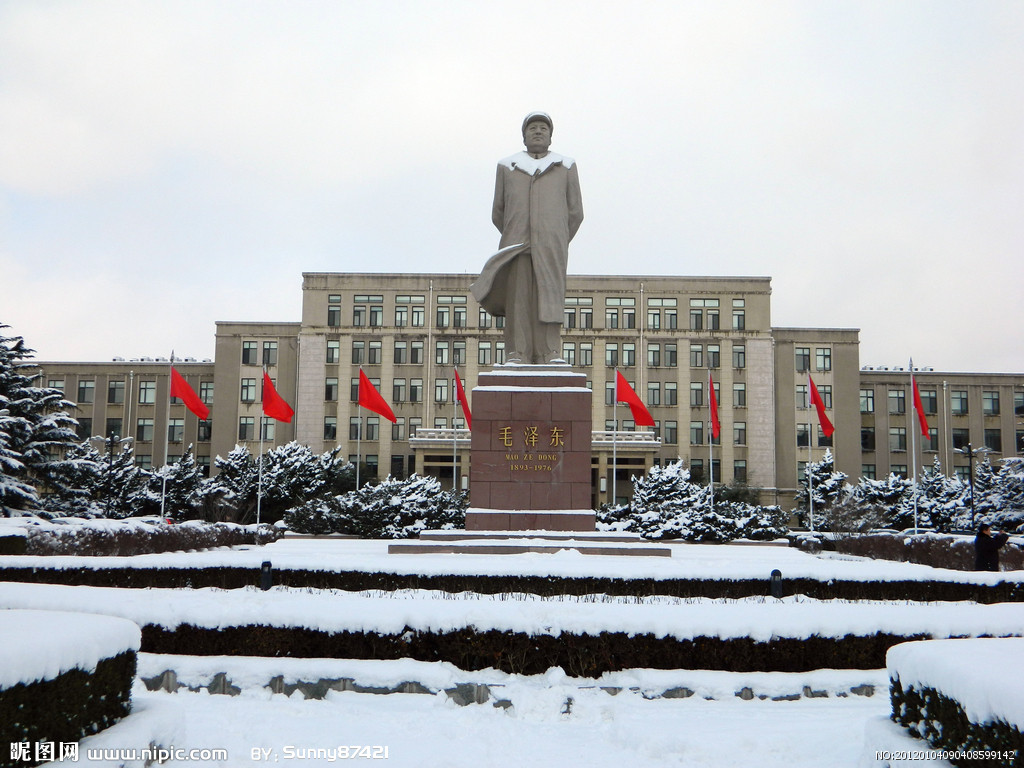
\includegraphics[width=0.8\linewidth]{figures/cmm.jpg}
    \bicaption[fig:cmm]{毛主席雕像}{毛主席像,请问主席举起哪一只手。}{Fig.}{Which hand of chirman Miao is up}
\end{figure}
表、图序号后面,同样适当留空(汉字状态敲两次空格键)。

图\ref{fig:cmm}显示了论文模板中所定义的样式选择方法。使用鼠标选择相应的样式,对应的文字格式就发生相应改变

\section{ 图的格式描述}
\esection{describe of figure format}
\begin{enumerate}[(1)]
\item 图的绘制方法
    \begin{asparaenum}[1)]
    \item 插图、照片应尽量通过扫描粘贴进本文。

    \item 简单文字图可用WORD直接绘制。
    \end{asparaenum}
\item 图的位置
    \begin{asparaenum}[1)]
    \item  图居中排列。

    \item 图与上文之间应留一空行。

    \item 图中若有附注,一律用阿拉伯数字和右半圆括号按顺序编排,如注1),附注写在图的下方。
    \end{asparaenum}
\item 图的版式
    \begin{asparaenum}[1)]
    \item “设置图片格式”的“版式”为“上下型”或“嵌入型”,不得“浮于文字之上”。

    \item 图的大小尽量以一页的页面为限,不要超限,一旦超限要加续图。
    \end{asparaenum}
\item 图名的写法
    \begin{asparaenum}[1)]
    \item 图名居中并位于图下,编号应分章编号,如图3.1。

    \item 图名与下文留一空行。

    \item 图及其名称要放在同一页中,不能跨接两页。

    \item 图内文字清晰、美观。

    \item 中文图名设置为黑体,小四号,居中。英文名称设置为Times New Roman,小四号,居中。 
    \end{asparaenum}
\end{enumerate}

\subsection{表的格式说明}
\esubsection{format of table}

\subsection{表格的格式示例}
\esubsection{example of table format}

表在正文中的常用格式如表3.1-3.3所示,使用三线表。

物流的概念和范围如表3.1表述。

表、图序号与后面文字同样应当适当留空(两次空格键)。
\begin{table}[h]
    \bicaption[tab:chap02:logistics]{物流的概念和范围}{物流的概念和范围}{Tab.}{Conception and scope of Logistics}
    \centering
    \vspace{0.2cm}
    \wuhao
    \begin{tabular}{cc}
    \hline
    {\hei 本质} & {\hei 过程}\\
    \hline
    途径或方法 & 规划、实施、控制\\
    目标 & {效率、成本效益}\\
    活动或作业 & 流动与储存\\
    处理对象 & 原材料、在制品、产成品、相关信息\\
    范围 & 从原点(供应商)到终点(最终顾客)\\
    目的或目标 & 适应顾客的需求(产品、功能、数量、质量、时间、价格)\\
    \hline
    \end{tabular}
\end{table}

美国广义物流后(勤)协会给出的定义如下:“为了符合顾客的要求,
从原点到消费点对原材料、在制品、产成品与相关信息的流动和
储存的效率成本效益进行规划、实施和控制的过程”。由此可见,
物流不是作为一种具体技术和方法来研究的,而是一个过程或管理。

\subsection{表的格式描述}
\esubsection{describe of table format}
\begin{enumerate}[(1)]
    \item  表的绘制方法

表要用WORD绘制,不要粘贴。如果要求使用Excel表格,则使用数值粘贴。
    \item   表的位置
	\begin{asparaenum}[1)]
       \item  表格居中排列。

       \item 表格与下文应留一行空格。

       \item 表中若有附注,一律用阿拉伯数字和右半圆括号按顺序编排,如注1),附注写在表的下方。
       \end{asparaenum}
    \item 表的版式
	\begin{asparaenum}[1)]
	\item 表的大小尽量以一页的页面为限,不要超限,一旦超限要加续表。
	\end{asparaenum}
    \item 表名的写法
    \begin{asparaenum}[1)]
	\item 表名应当在表的上方并且居中。编号应分章编号,如表3.1、表3.2。

	\item 表名与上文留一空行。

	\item 表及其名称要放在同一页中,不能跨接两页。

	\item 表内文字全文统一,设置为宋体,五号。

	\item 中文表名设置为宋体,小四号,且居中。英文名称设置为Times New Roman,小四号,且居中。
    \end{asparaenum}

\end{enumerate}

\section{公式的格式说明}
\esection{formula format}%
\label{sec:formula_format}
\subsection{公式格式示例}
\esubsection{example for formula}
由于一般的文献资料中所给出的载荷和抗力的统计参数主要为变异系数,为便于讨论,定义公式形式如下:
\begin{equation}
    \textrm{LRI} = 1  \bigg / \sqrt{1 + \qty (\frac{\mu_R}{\mu_s})^2 \qty (\frac{\delta_R}{\delta_S})^2 }
    \label{Eq:31}
\end{equation}
其中,$\mu_R, \mu_S$分别为抗力和载荷的均值\dots 。

\subsection{公式的格式描述}
\esubsection{describe of math format}

\begin{asparaenum}[(1)]
\item 公式整行右对齐,并调整公式与公式序号之间的距离,使公式部分居中显示。

\item 公式序号应按章编号,公式编号在行末列出,如 \eqref{Eq:31}。

\item 公式位置:公式之间及上下文间设置半行间距或者6磅,作者可根据情况适当调整,以保证格式协调和美观。
\end{asparaenum}

\section{参考文献的格式说明}
\esection{explain of format of reference}

\subsection{参考文献在正文中引用的示例}
\esubsection{example for citation}
大连理工大学的量子力学课程使用宋鹤山老师的教材\cite{BOOK.hssong2006},
也可以参考张永德老师的高等量子力学教材\cite{BOOK.Zhang2009}

% vim: set textwidth=80:
% vim: set formatoptions+=m:
\chapter{\TeX 使用技巧}
\echapter{Skills of \TeX}
\begin{Sketch}
    本章主要给出本模板中有用的一些技巧,能为编写论文提供极大的方便。
\end{Sketch}
\section{编译}
\esection{compile}
\label{sec:compile}
    \XeLaTeX 可以很好的支持中文,引入中文字体极为方便,是中文\TeX 的优秀引擎,
    本模板使用\XeLaTeX 。

推荐论文每章放置在一个独立的tex文件中,然后使用\verb|\include|命令导入,为了提高
编译速度,可以在导言区使用 
\begin{lstlisting}
\includeonly{<tex file1>,<tex file2>,...}
\end{lstlisting}
来分段编译。

\section{字体}
\esection{font}
\label{sec:font}
    字体文件在目录font中,如果有需要也可以在模板文件
    dutthesis.cls 中修改字体部分,选择需要的字体。
    \begin{lstlisting}[language=TeX]
	\setmainfont[
	Path = ./font/,
	BoldFont=timesbd.ttf,
	ItalicFont=timesi.ttf,
	BoldItalicFont=timesbi.ttf
	]{times.ttf}


	% 修改中文字体族,增加黑体
	\setCJKmainfont[
	Path = ./font/,
	BoldFont=simhei.ttf,
	ItalicFont=simkai.ttf,
	BoldItalicFont=simfang.ttf
	]{simsun.ttc}
	\setCJKfamilyfont{zhsong}[Path = ./font/]{simsun.ttc}
	\newcommand{\song}{\CJKfamily{zhsong}}
	\setCJKfamilyfont{zhhei}[Path = ./font/]{simhei.ttf}
	\newcommand{\hei}{\CJKfamily{zhhei}}
	\setCJKfamilyfont{FZXiHei}[Path = ./font/]{FZXH1K.TTF}
	\newcommand{\xhei}{\CJKfamily{FZXiHei}}
	\setCJKfamilyfont{zhkai}[Path = ./font/]{simkai.ttf}
	\newcommand{\kai}{\CJKfamily{zhkai}}
	\setCJKfamilyfont{zhfs}[Path = ./font/]{simfang.ttf}
	\newcommand{\fs}{\CJKfamily{zhfs}}
	\setCJKfamilyfont{FZXingKai}[Path = ./font/]{FZXKK.TTF}
	\newcommand{\xkai}{\CJKfamily{FZXingKai}}
    \end{lstlisting}
当然为了方便也可以使用本机字体。



\section{交叉引用}
\esection{corss reference}
\label{sec:cross-reference}
在论文中往往需要对章节、图表、公式进行引用,\LaTeX 编写论文基本依赖于hyperref包
实现引用。

本模板中推荐使用\verb|\autoref{<the label>}| 交叉引用,其中autoref的相关设置位于
dutthesis-utf8.cfg中
\begin{lstlisting}[language=TeX]
    \renewcommand{\figureautorefname}{图}
    \renewcommand{\tableautorefname}{表}
    \renewcommand{\figurename}{图}
    \def\equationautorefname#1#2\null{方程#1(#2\null)}
    \def\chapterautorefname#1#2\null{第#1#2 章}
    \def\subsectionautorefname#1#2\null{#1#2 小节}
    \def\sectionautorefname#1#2\null{#1#2 节}
\end{lstlisting}
基于这些设置,可以很好的实现交叉引用,而且不需要作者对被引用对象的识别,计算机将
分别对章节、图表、公式加以不同的表述,如:
\begin{lstlisting}[language=TeX]
    \autoref{cha:format},
    \autoref{sec:advance},
    \autoref{fig:cmm},
    \autoref{Eq:31},
\end{lstlisting}
\autoref{cha:format},
\autoref{sec:advance},
\autoref{fig:cmm},
\autoref{Eq:31},
当然\verb|\ref \eqref|等方式依旧可以使用,只是相对不如autoref方便。

hyperref包可以通过命令 \verb|\hypersetup{× = ×}| 设置引用连接的格式,使用本模
板时,可以通过 \verb|\documentclass[hidelinks]{dutthesis}| 选择无格式的交叉
引用。

\section{参考文献}
\esection{reference}
\label{sec:reference}
本模板使用bibtex引用参考文献,请将需要引用的文献放置于bib文件中
在需要引用的地方使用\verb|\cite{<keys>}|引用(上标),可以使用
\verb|\citet{<keys>}| 实现行内引用。

在正文中使用Reference环境输出参考文献
\begin{lstlisting}[language=TeX]
\begin{Reference}
\bibliography{<bib file>}
\end{Reference}
\end{lstlisting}
请记得添加Reference环境!

本参考文献样式使用\hyperlink{https://github.com/zepinglee/gbt7714-bibtex-style}
{gbt7714-bibtex-style},该样式可定制性强,arXiv支持做的还可以。我并对其中的gbt7714-numberical.bst做了一定修改,有需要可根据文档修改
\begin{lstlisting}[language=TeX]
FUNCTION {load.config}
{
  #2 'citation.et.al.min :=
  #1 'citation.et.al.use.first :=
  #4 'bibliography.et.al.min :=
  #3 'bibliography.et.al.use.first :=
  #1 'uppercase.name :=
  #0 'terms.in.macro :=
  #0 'year.after.author :=
  #1 'period.after.author :=
  #0 'italic.book.title :=
  #1 'sentence.case.title :=
  #1 'link.title :=
  #1 'title.in.journal :=
  #0 'show.patent.country :=
  #1 'show.mark :=
  #0 'space.before.mark :=
  #1 'show.medium.type :=
  "slash" 'component.part.label :=
  #0 'short.journal :=
  #1 'italic.journal :=
  #1 'bold.journal.volume :=
  #0 'show.missing.address.publisher :=
  #1 'space.before.pages :=
  #1 'only.start.page :=
  #0 'wave.dash.in.pages :=
  #1 'show.urldate :=
  #0 'show.url :=
  #0 'show.doi :=
  #1 'show.preprint :=
  #0 'show.note :=
  #0 'show.english.translation :=
  #1 'end.with.period :=
}
\end{lstlisting}
效果见\hyperref[cha:reference]{参考文献}
\section{章节、目录以及相关杂项}
\esection{chapter,section, contents and others}
\label{sec:Chapter-section-contents-others}
本节包含章节、目录以及其格式设定等问题。
\subsection{章节}
\esubsection{chapter and section}%
\label{sub:chapter-section}
为了实现双语目录,新章节都需要引入响应的英语章节。
\begin{table}[h]
    \bicaption[tab:chapter-sections]{中英文章节}{中英文章节命令对照表格,中文名
	在autoref中也有设定,见\autoref{sec:cross-reference}。
    }{Tab.}{The command of Chinese and english chapter and sections}
    \centering
    \begin{tabular*}{0.85\textwidth}{@{\extracolsep{\fill}}ccc}
	\hline
     中文名& 中文命令 & 英文命令 \\ \hline
     章 & \verb|\chapter[toc name]{chapter name}| & \verb|\echapter{toe name}| \\ \hline
     节 & \verb|\section| & \verb|\esection| \\ \hline
     小节 & \verb|\subsection| & \verb|\esubsection| \\ \hline
    \end{tabular*}
\end{table}
英文标题用于生成英文目录,硕士不需要英文目录,因此可以不要英文章节命令。

\subsection{目录}
\esubsection{contents}%
\label{sub:contents}
中文目录使用\verb|\tableofcontents| 生成,英文目录\verb|\tableofengcontents|,
图表目录\verb|\tableoffigurecontents,\tableoftablecontents|(这个需要存在英文目
录才行),或者也可以使用\verb|\listoffigures|, \verb|\listoftable|。
实际上只有博士需要英文,图表目录。

\subsection{杂项}
\esubsection{others}%
\label{sub:others}
摘要使用环境abstract, 英文摘要englishabstract,同时abstract环境附带了关键词选项
\begin{lstlisting}[language=TeX]
   \begin{abstract}{keywords,...}
       .....
   \end{abstract} 
   \begin{englishabstract}{english keywords, ....}
       .....
   \end{englishabstract}
\end{lstlisting}

尽管学校的模板中没有对每章正文之前加入摘要,或者简述,遵照过往的经验,依旧定义了
一个Sketch环境来引入章节简述。

发表论文情况使用环境Publics。

致谢定义了环境 Acknowledgement。

博士论文需要有个人简历,使用环境Resume。
\begin{lstlisting}[language=TeX]
    \begin{Resume}
	\begin{minipage}{0.8\textwidth}
		\linespacing{1.6}
	    \begin{tabular}{lp{2\baselineskip}}
		姓名:  三分先生\\
		性别: 男\\
		出生年月:  1991 年 7 月  \\
		民族:  汉 \\
		籍贯:  灵台方寸山,斜月三星洞\\
		研究方向: \LaTeX  以及 \XeLaTeX\\
		简历:\\
	    \end{tabular}
	\end{minipage}
	\begin{minipage}{0.2\textwidth}
	    \flushright
	    \vspace*{-80pt}
		\fboxrule=1.2pt \fboxsep=0pt
		\fcolorbox{gray}{white}{
		     
\includegraphics[width=3.5cm,height=5cm]{figures/doctor-hwzs.pdf}
	    }
    \end{minipage}

    三分先生不知何许人也,其人额大颡突,发线高耸,额雄踞头部三分,乃以三分为号。
    人或曰,昔者杜甫诗云,``功盖三分国,名称八卦图",
    如此先生岂非有孔明之大志,怀管乐之奇才乎?
    非也,乱世雄图,与治世而何?故无其才,安能谋事。
    天下当混为一,安可分!三分者,徒先生之怪貌者也。
    $\ldots \cdots$
    \end{Resume}
\end{lstlisting}


% vim: set textwidth=80:
% vim: set formatoptions+=m:
\chapter{不同学位情况说明}
\echapter{details for different degrees}
本模板优先支持大连理工大学博士学位论文。
当选择了不同学位,\verb|\@degree| 将会设定成学位类型,硕士、博士等等。
学校名在dutthesis.cfg中定义,\verb|\universityname|英文名也在其中。
(\universityname\makeatletter\@degree\makeatother)
\section{博士学位论文}
\esection{doctor thesis}
\begin{lstlisting}[language=TeX]
    \documentclass[doctor]{dutthesis} %其他选项也可添加
\end{lstlisting}

大连理工大学论文模板结构比较混乱,比如标题的格式,加粗不加粗都存在一定争议,本论文中居中标题没有加粗,如果有需要可以自己添加(没必要)。
此外应该注意博士论文中,独创性声明与版权声明在同一页,模板已经处理好。
其中独创性声明命令为\verb|\declare|,
对于博士论文来说,\verb|\declare|包含了版权声明\verb|\dutauthorization|命令(见
dutthesis-utf8.cfg)。

博士论文中英文摘要不进入目录,目录第一条为绪论,且需要加入英文目录,图、表目录。
本模板中博士论文可以依次使用命令
\begin{lstlisting}[language=TeX]
\tableofcontents
\tableofengcontents
\cleardoublepage
\tableoffigurecontents
\tableoftablecontents
\end{lstlisting}
其中 \lstinline|\cleardoublepage| 用于清空页面到奇数页,而
\lstinline|\tableofengcontents, \tableoffigurecontents, \tableoftablecontents|为
(重)新定义的各类目录,这里如果不使用英文目录,则图表目录也不能用上述命令,
但是 \lstinline|\listoffigures,\listoftables|依旧可以使用,会导致图表目录都另启
一页。

博士论文需要填写主要符号表这一页,范例如下:
\begin{lstlisting}[language=TeX]
\subcapter{主要符号}

\begin{table}[H]
%\bicaption[table]{主要符号表}{}
%{Tab.}{}
%根据学校给出的模板,主要符号表为单独一章,表头无序号,不计入“表目标”中  李2018.3
\begin{center}
\begin{tabular}{ccc}
  \hline
  % after \\: \hline or \cline{col1-col2}  ...
  符号          & 代表意义     & 单位  \\
  $T$   & 温度     & K \\
  $m$   & 质量     & kg \\
  $L$   & 长度     & m \\
  $\kappa$   & 光场耗散     & Hz \\
  $\omega$   & 频率     & Hz \\
  $\omega_{m}$   & 机械振子频率     & Hz \\
  $\gamma_{m}$   & 机械振子耗散率     & Hz \\
  $g$   & 光力耦合强度     & Hz \\
  $\hbar$   & 约化普朗克常数(如未特别强调,取$\hbar=1$)     & J$\cdot$ s  \\
  $k_B$  & 玻尔兹曼常数     & J/K \\
  $\langle\dots\rangle$   & 取量子态下期望值     & \\
  $\delta(\dots)$   & 狄拉克函数     & \\ 
  $\delta_{ij}$   & 克罗内克符号     & \\ 
  $H_{\textrm{eff}}$   & 有效哈密顿量     & \\ 
  $H_{\textrm{int}}$   & 相互作用哈密顿量     & \\ 
  $H_{\textrm{tot}}$   & 总哈密顿量     & \\ 
\end{tabular}
\end{center}
\end{table}
\end{lstlisting}

成果页面使用定制的Publics环境,定义代码如下:
\begin{lstlisting}[language=TeX]
    \newenvironment{Publics}[1][\@publicstitle]
    {%
      \stcleardp
      \phantomsection
      \addcontentsline{toc}{chapter}{\@publicstitletoc}
      \subchapter*{#1}
      \addcontentsline{toe}{chapter}{Achievements}
      \song\xiaosihao
    }{\par}
\end{lstlisting}
博士的科研成果页面将根据学位而自动修改。
主要配置为:
\begin{lstlisting}[language=TeX]
\newcommand{\@publicstitle}{攻读\@degree 学位期间科研项目及科研成果}
\newcommand{\@publicstitletoc}{攻读\@degree 学位期间科研项目及科研成果}
\end{lstlisting}

博士论文需要加入个人简介页面,模板重新定义了Resume环境。
范例如下:
\begin{lstlisting}[language=TeX]
 \begin{Resume}
    \begin{minipage}{0.8\textwidth}
	    \linespacing{1.6}
	\begin{tabular}{lp{2\baselineskip}}
	    姓名:  三分先生\\
	    性别: 男\\
	    出生年月:  1991 年 7 月  \\
	    民族:  汉 \\
	    籍贯:  灵台方寸山,斜月三星洞\\
	    研究方向: \LaTeX  以及 \XeLaTeX\\
	    简历:\\
	\end{tabular}
    \end{minipage}
    \begin{minipage}{0.2\textwidth}
	\flushright
	\vspace*{-80pt}
	    \fboxrule=1.2pt \fboxsep=0pt
	    \fcolorbox{gray}{white}{
		 
\includegraphics[width=3.5cm,height=5cm]{figures/doctor-hwzs.pdf}
		 %插入照片
	}
\end{minipage}

三分先生不知何许人也,其人额大颡突,发线高耸,额雄踞头部三分,乃以三分为号。
人或曰,昔者杜甫诗云,``功盖三分国,名称八卦图",
如此先生岂非有孔明之大志,怀管乐之奇才乎?
非也,乱世雄图,与治世而何?故无其才,安能谋事。
天下当混为一,安可分!三分者,徒先生之怪貌者也。
$\ldots \cdots$
\end{Resume}   
\end{lstlisting}

\section{硕士学位论文}
\esection{master thesis}
\begin{lstlisting}[language=TeX]
    \documentclass[master]{dutthesis} %其他选项也可添加
\end{lstlisting}
硕士论文与博士稍有不同。

独创性声明页面不包括版权声明,版权声明在最后一页。

硕士论文只有中文目录,且中英文摘要都要进入目录。

硕士论文的Introduction定义了新环境,因为格式特殊,所以要在Introduction环境中写,
坑爹啊!!!

硕士论文有一章为结论,定义了Conclusion环境,博士模板无此环境!!!
\begin{lstlisting}[language=TeX]
%%%%%%%%%%%%%%%
%  结论环境,硕士需要  %
%%%%%%%%%%%%%%%
\ifmasterdegree
\newenvironment{Conclusion}
{%
  \stcleardp
  \phantomsection
  \addcontentsline{toc}{chapter}{结论}
  \subchapter*{结论}
  \addcontentsline{toe}{chapter}{conclusion}
  \song \xiaosihao
}{\par}
\fi
\end{lstlisting}

硕士论文发表情况页面自动根据 \lstinline|\@degree| 修改,选择硕士论文选项就好。

硕士论文的版权页面将自动生成,为最后一页。
\section{学士学位}
\esection{bachelor}
Waiting

\end{Main} % 结束正文
\begin{Appendix}
    \chapter{附录的工作原理}
    \echapter{Mechanism of Appendix}
    附录放置于Main环境之外!!
    这里附录通过引用Appendix环境使用,具体环境定义为:
    \begin{lstlisting}[language=TeX]
	\newenvironment{Appendix}
	{
	  \pagestyle{dutstyle}
	  \@mainmattertrue
	  \appendix
	  %\titlecontentsappendix
	}{\@mainmatterfalse\par
	  \thispagestyle{dutstyle}\clearpage
	}
    \end{lstlisting}


    \section{附录的特点}
    由于使用了 \lstinline|\appendix|命令,因此附录之后章节计数器将清空并改用字母标记!! 
    \chapter{目录中的附录以及特点}
    为了写作方便,附录中的章、节命令不变依旧是 \lstinline|\chapter \section ...|,但是这给编写论文带来一定难度,因此这里做了些小聪明的修改。
    \section{目录中的附录}
    根据学校要求,目录中附录应该与章地位相同,但是目录标记不同。
    在这里通过对章的计数器形状判别,如果为 \lstinline|\AppendixListAlph|中定义的字母则该章为附录,按照特殊格式排版。 
    部分代码如下:
    \begin{lstlisting}[language=TeX]
	\titlecontents{chapter}[0pt]{\song \xiaosihao}
	{\IfSubStr{\AppendixListAlph}{\thecontentslabel}{\contentslabel[\AppendixTOCName~\thecontentslabel]{0mm}\phantom{\AppendixTOCName~\thecontentslabel}\quad}{\thecontentslabel\quad}}{}
	{\titlerule*[5pt]{.}\thecontentspage}  %判断chapter计数器是否为字母,字母则为附录
	\titlecontents{subchapter}[0pt]{\song \xiaosihao}
	{}{}
	{\quad\titlerule*[5pt]{.}\thecontentspage}
    \end{lstlisting}
    这类附录目录格式修改对于中英文目录都要特殊处理。

    \section{附录标题}
    附录标题居中,因此本模板将根据之前的计数器判别法判别某章是否为附录,如果为附录重新定义目录格式:
    \begin{lstlisting}[language=TeX]
	    \titleformat{\chapter}[hang]{\IfSubStr{\AppendixListAlph}
	    {\thechapter}{\centering}{}
	    \hei \xiaosanhao \linespacing{1.5}}{\chaptertitlename}{1em}{}%黑体 小三
    \end{lstlisting}
\end{Appendix}
\begin{Reference}
\bibliography{bibtex.bib}
\end{Reference}
\begin{Publics}
    首先列出博士生攻读博士学位期间发表(含已录用)与学位论文有关的学术论文,并注明属于学位论文内容的部分(章节),作者(最多三个)、论文题目、刊物名称、时间、卷期号、页码以及检索信息、与学位论文相关章节。其他时间或与学位论文内容(章节)无关的论文不得列出。

其次列出在攻读博士学位期间参与的科研项目(如国家自然科学基金或国家“863”计划等),以及在这期间取得的科研成果(申请的发明专利、科研奖励等)。

书写格式说明:

标题“攻读博士学位期间科研项目及科研成果”选用模板中的样式所定义的“发表学术论文情况”;或者手动设置成字体:黑体,居中,字号:小三,1.5倍行距,段后1行,段前为0行。

“攻读博士学位期间科研项目及科研成果”正文选用模板中的样式所定义的“正文”,每段落首行缩进2字;或者手动设置成每段落首行缩进2字,字体:宋体,字号:小四,行距:多倍行距 1.25,间距:前段、后段均为0行。

例:

发表论文

[1] DesES MaraisARAIS D. J., Strauss TRAUSS H. , SummonsUMMONS R. E., et al. Carbon isotope evidence for the stepwise oxidation of the Proterozoic environment [J]. Nature, 1992,359:605-609. (SCI检索号:123DX) (本学位论文第一章)
~\\

参与科研项目

[1] 国家自然科学基金项目(51276055):西南喀斯特山区土地利用和土地覆被变化及其对土地资源可持续性影响研究,2013.1 – 2016.12,负责人:爱因斯坦。
~\\

发明专利

[1] 发明人1,发明人2,发明人3. 多功能一次性压舌板:中国,92214985.2[P]. 发明类别:发明专利,公开(或授权)日期:1993,04,14.
~\\


获得奖励

[1] “大型C/E复合材料构件高质高效加工关键技术及其工艺装备”,机械工业科学技术奖-科技进步一等奖,2013.10, 总排序1。
\end{Publics}
\begin{Acknowledgement}
    学位论文中不得书写与论文工作无关的人和事(可以写家人),对导师的致谢要实事求是。

一同工作的同志对本研究所做的贡献应在论文中做明确的说明并表示谢意。

这部分内容不可省略。

书写格式说明:

标题“致谢”选用模板中的样式所定义的“致谢”;或者手动设置成字体:黑体,居中,字号:小三,1.5倍行距,段后1行,段前为0行。

致谢正文选用模板中的样式所定义的“正文”,每段落首行缩进2字;或者手动设置成每段落首行缩进2字,字体:宋体,字号:小四,行距:多倍行距 1.25,间距:前段、后段均为0行。
\end{Acknowledgement}

\begin{Resume}
    \begin{minipage}{0.8\textwidth}
	    \linespacing{1.6}
	\begin{tabular}{lp{2\baselineskip}}
	    姓名:  三分先生\\
	    性别: 男\\
	    出生年月:  1991 年 7 月  \\
	    民族:  汉 \\
	    籍贯:  灵台方寸山,斜月三星洞\\
	    研究方向: \LaTeX  以及 \XeLaTeX\\
	    简历:\\
	\end{tabular}
    \end{minipage}
    \begin{minipage}{0.2\textwidth}
	\flushright
	\vspace*{-80pt}
	    \fboxrule=1.2pt \fboxsep=0pt
	    \fcolorbox{gray}{white}{
		 
\includegraphics[width=3.5cm,height=5cm]{figures/doctor-hwzs.pdf}
	}
\end{minipage}

三分先生不知何许人也,其人额大颡突,发线高耸,额雄踞头部三分,乃以三分为号。
人或曰,昔者杜甫诗云,``功盖三分国,名称八卦图",
如此先生岂非有孔明之大志,怀管乐之奇才乎?
非也,乱世雄图,与治世而何?故无其才,安能谋事。
天下当混为一,安可分!三分者,徒先生之怪貌者也。
$\ldots \cdots$
\end{Resume}
\authorizationpage
% 参考文献}
%\bibliographystyle{GBT7714-2005NLang}
\newpage
\printindex % 索引

%\begidex % 索引n{thebibliography}{99}
%\bibliographystyle{ieee}
%\bibliography{seuthesis}
\end{document}
